% Provenance (never printed): cycle 2 "Explorer les organisations du monde ---
% identifier des paysages" (littoraux, massifs montagneux, campagnes, villes),
% see sources/book1/PROVENANCE.md. Book 1, grade 1, chapter 2.
\chapter{Landscapes Around Us}\label{ch:g1:landscapes-around-us}

Mia and her grandfather have walked all the way up the \omterm{def:g1:landscapes-around-us:landform}{hill} behind the
village. At the top they sit on the grass to catch their breath, and they
look. Below them, the red roofs of the village crowd around the church. A
\omterm{def:g1:landscapes-around-us:water}{river} winds between green and yellow fields and passes under a bridge.
There is a dark forest on the next \omterm{def:g1:landscapes-around-us:landform}{hill}. And far, far away, at the very end
of the land, there is a thin line of blue.

``That is the sea,'' says her grandfather.

Everything Mia can see from the top of the \omterm{def:g1:landscapes-around-us:landform}{hill}, near and far, is a
\omterm{def:g1:landscapes-around-us:landscape}{landscape}.

\begin{omfigure}
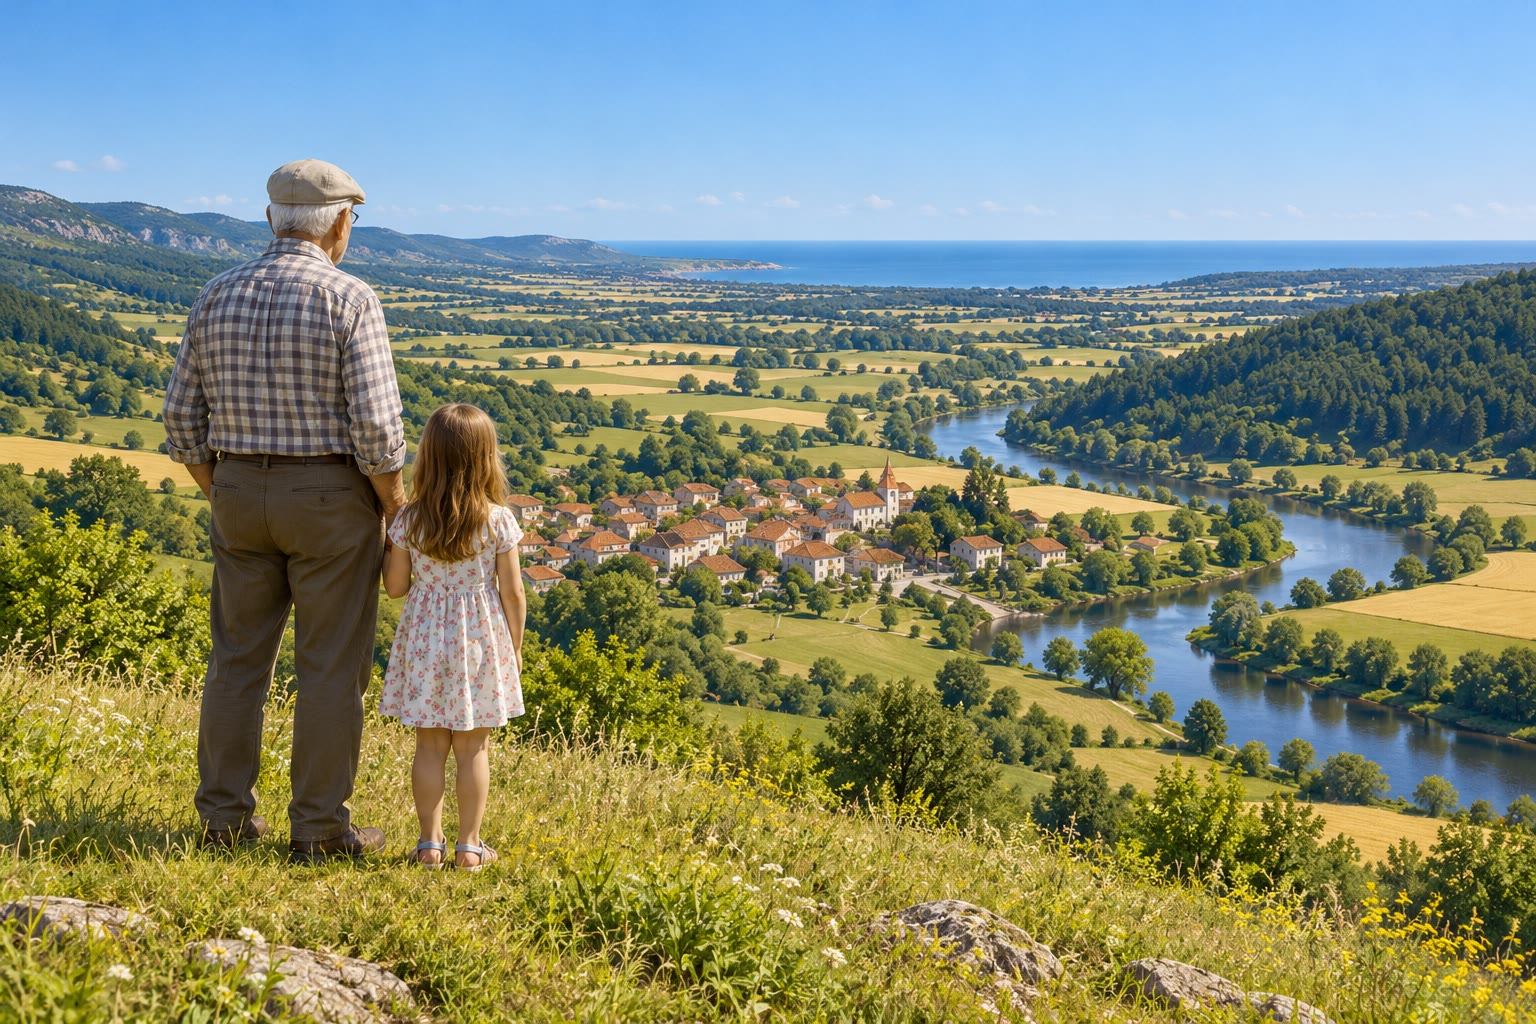
\includegraphics[width=0.72\linewidth]{images/book1/ai/g1-hilltop-view.jpg}

{\small From the top of a \omterm{def:g1:landscapes-around-us:landform}{hill} we see a whole \omterm{def:g1:landscapes-around-us:landscape}{landscape}.}
\end{omfigure}

\section{What is a landscape?}

\begin{definition}[Landscape]\label{def:g1:landscapes-around-us:landscape}
A \emph{landscape}\index{landscape} is everything we can see of the land in
one look, from where we stand to the far horizon: the shape of the ground,
the water, the plants, and the things people have built.
\end{definition}

A \omterm{def:g1:landscapes-around-us:landscape}{landscape} has parts that are near and parts that are far. The part
nearest to us is at the bottom of what we see; it looks big and we see its
details. The far part is at the top, close to the sky; it looks small and
pale.

\begin{omfigure}
\begin{tikzpicture}[x=1cm, y=1cm]
  \fill[ocBlue!12] (0,0) rectangle (10,5);
  % background: far hills
  \fill[black!18] (0,3.0) -- (1.5,3.6) -- (3,3.3) -- (5,3.9) -- (7,3.4) -- (8.5,3.8) -- (10,3.3) -- (10,2.9) -- (0,2.9) -- cycle;
  % middle: hills and fields
  \fill[green!35!omLithAlluv] (0,1.6) -- (2,2.4) -- (4,2.1) -- (6,2.7) -- (8,2.2) -- (10,2.5) -- (10,1.5) -- (0,1.5) -- cycle;
  \fill[green!25!omLithAlluv] (0,1.5) rectangle (10,2.95);
  \fill[green!35!omLithAlluv] (0,2.95) -- (2,3.1) -- (4,2.95) -- (6,3.25) -- (8,3.0) -- (10,3.1) -- (10,2.9) -- (0,2.9) -- cycle;
  \foreach \x in {5.6,5.9,6.2} \fill[red!55] (\x,2.25) -- ++(0.12,0.15) -- ++(0.12,-0.15) -- cycle;
  \foreach \x in {5.6,5.9,6.2} \fill[white] (\x+0.03,2.1) rectangle ++(0.18,0.15);
  % foreground
  \fill[green!55!black!60] (0,0) rectangle (10,1.5);
  \foreach \x in {0.8,2.1,8.6} {
    \fill[brown!70!black] (\x-0.06,0.4) rectangle (\x+0.06,0.9);
    \fill[green!45!black] (\x,1.15) circle (0.38);
  }
  % band borders and labels
  \draw[white, line width=1pt, dashed] (0,1.5) -- (10,1.5);
  \draw[white, line width=1pt, dashed] (0,2.95) -- (10,2.95);
  \node[font=\small\bfseries, fill=white, fill opacity=0.8, text opacity=1, inner sep=2pt] at (5,0.6) {foreground: near, big, many details};
  \node[font=\small\bfseries, fill=white, fill opacity=0.8, text opacity=1, inner sep=2pt] at (2.7,2.2) {middle ground};
  \node[font=\small\bfseries, fill=white, fill opacity=0.8, text opacity=1, inner sep=2pt] at (5,4.4) {background: far, small, pale};
\end{tikzpicture}

{\small A \omterm{def:g1:landscapes-around-us:landscape}{landscape} seen in three bands: the foreground at the bottom, the
middle ground, and the background against the sky.}
\label{fig:g1:landscapes-around-us:bands}
\end{omfigure}

\section{The shapes of the land}

The ground is not flat everywhere. In some places it rises high into the
sky; in others it goes down into long hollows; elsewhere it is flat as far
as we can see. We give a name to each shape.

\begin{definition}[Landforms]\label{def:g1:landscapes-around-us:landform}
A \emph{landform}\index{landform} is a shape of the land's surface.
\begin{itemize}
  \item A \emph{mountain}\index{mountain} is a very high landform with steep
        slopes; its top is called the summit. The highest mountains have
        snow on top even in summer.
  \item A \emph{hill}\index{hill} is a landform that rises above the land
        around it, lower and rounder than a mountain.
  \item A \emph{valley}\index{valley} is a long, low hollow between hills or
        mountains; there is often a \omterm{def:g1:landscapes-around-us:water}{river} at the bottom.
  \item A \emph{plain}\index{plain} is a wide, flat, low stretch of land.
\end{itemize}
\end{definition}

\begin{omfigure}
\begin{tikzpicture}[x=1cm, y=1cm]
  \fill[ocBlue!10] (0,0) rectangle (12.4,4.6);
  % sea
  \fill[omSea] (10.2,0) rectangle (12.4,0.55);
  % land profile: mountains, valley, hill, plain, coast
  \fill[omLithAlluv!80!green] (0,0) -- (0,2.2) -- (0.9,3.3) -- (1.5,3.0) -- (2.2,4.1)
     -- (2.9,2.6) -- (3.6,1.2) -- (3.9,0.9) -- (4.2,1.2) -- (5.0,2.0) -- (5.7,2.2)
     -- (6.4,1.6) -- (7.0,0.95) -- (8.0,0.8) -- (9.5,0.7) -- (10.2,0.6) -- (10.4,0.55)
     -- (10.4,0) -- cycle;
  \draw[black!60, line width=0.6pt] (0,2.2) -- (0.9,3.3) -- (1.5,3.0) -- (2.2,4.1)
     -- (2.9,2.6) -- (3.6,1.2) -- (3.9,0.9) -- (4.2,1.2) -- (5.0,2.0) -- (5.7,2.2)
     -- (6.4,1.6) -- (7.0,0.95) -- (8.0,0.8) -- (9.5,0.7) -- (10.2,0.6) -- (10.4,0.55);
  % snow caps
  \fill[white, draw=black!50, line width=0.3pt] (1.95,3.72) -- (2.2,4.1) -- (2.45,3.72) -- (2.3,3.78) -- (2.2,3.68) -- (2.08,3.78) -- cycle;
  \fill[white, draw=black!50, line width=0.3pt] (0.72,3.08) -- (0.9,3.3) -- (1.05,3.15) -- (0.9,3.12) -- cycle;
  % river in the valley
  \fill[omSea!90!black] (3.75,0.92) rectangle (4.05,0.98);
  % lake on the plain
  \fill[omSea] (7.6,0.82) ellipse (0.5 and 0.07);
  % village on the plain
  \foreach \x in {8.6,8.85,9.1} {
    \fill[white, draw=black!50, line width=0.3pt] (\x,0.74) rectangle ++(0.18,0.16);
    \fill[red!60] (\x-0.02,0.9) -- ++(0.11,0.12) -- ++(0.11,-0.12) -- cycle;
  }
  % labels
  \node[font=\small, above] at (2.2,4.12) {mountain};
  \node[font=\small, above] at (5.6,2.25) {hill};
  \node[font=\small] at (3.9,1.85) {valley};
  \node[font=\small, above] at (8.2,1.5) {plain};
  \draw[black!60, thin] (8.2,1.5) -- (8.2,0.85);
  \node[font=\small, align=center] at (11.3,1.4) {sea};
  \node[font=\scriptsize, below=2pt, fill=white, fill opacity=0.8, text opacity=1, inner sep=1pt] at (7.6,0.35) {lake};
  \draw[black!60, thin] (7.6,0.45) -- (7.6,0.78);
  \node[font=\scriptsize, below=2pt, fill=white, fill opacity=0.8, text opacity=1, inner sep=1pt] at (10.3,0.35) {coast};
  \node[font=\scriptsize, fill=white, fill opacity=0.8, text opacity=1, inner sep=1pt] at (3.9,0.2) {river};
  \draw[black!60, thin] (3.9,0.32) -- (3.9,0.88);
\end{tikzpicture}

{\small The shapes of the land, from the \omterm{def:g1:landscapes-around-us:landform}{mountains} to the sea, seen from
the side (the heights are drawn much taller than they really are).}
\label{fig:g1:landscapes-around-us:profile}
\end{omfigure}

\begin{omfigure}
\begin{minipage}[b]{0.49\linewidth}\centering
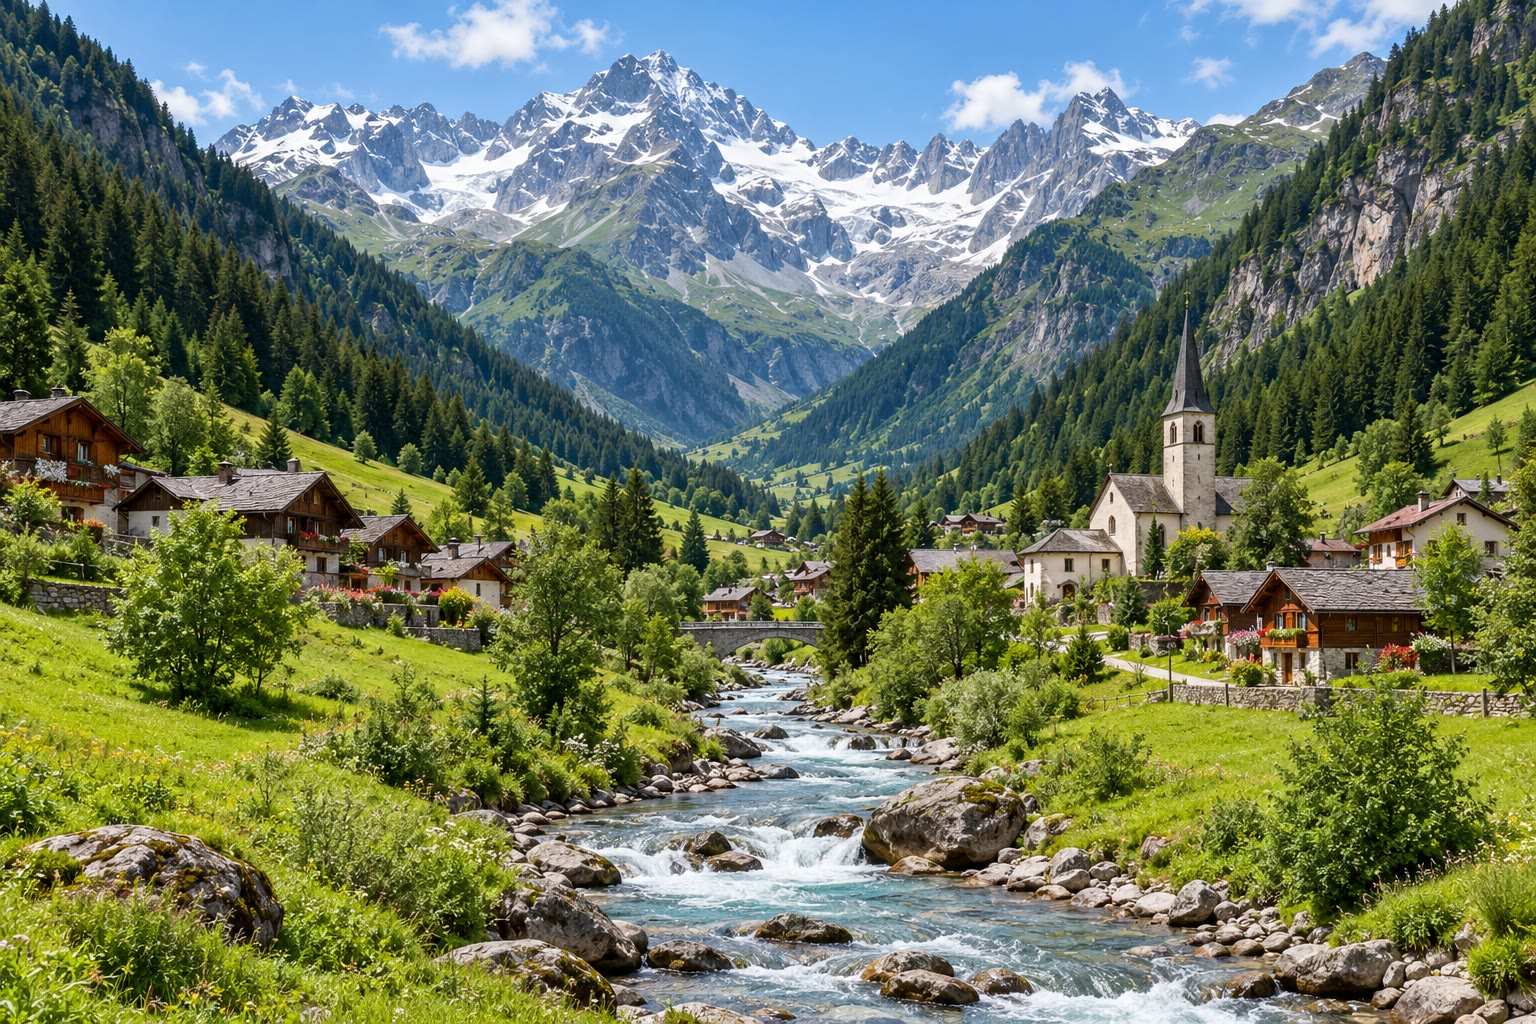
\includegraphics[width=\linewidth]{images/book1/ai/g1-mountain-village.jpg}

{\small \omterm{def:g1:landscapes-around-us:landform}{Mountains}, and a village in their \omterm{def:g1:landscapes-around-us:landform}{valley}.}
\end{minipage}\hfill
\begin{minipage}[b]{0.49\linewidth}\centering
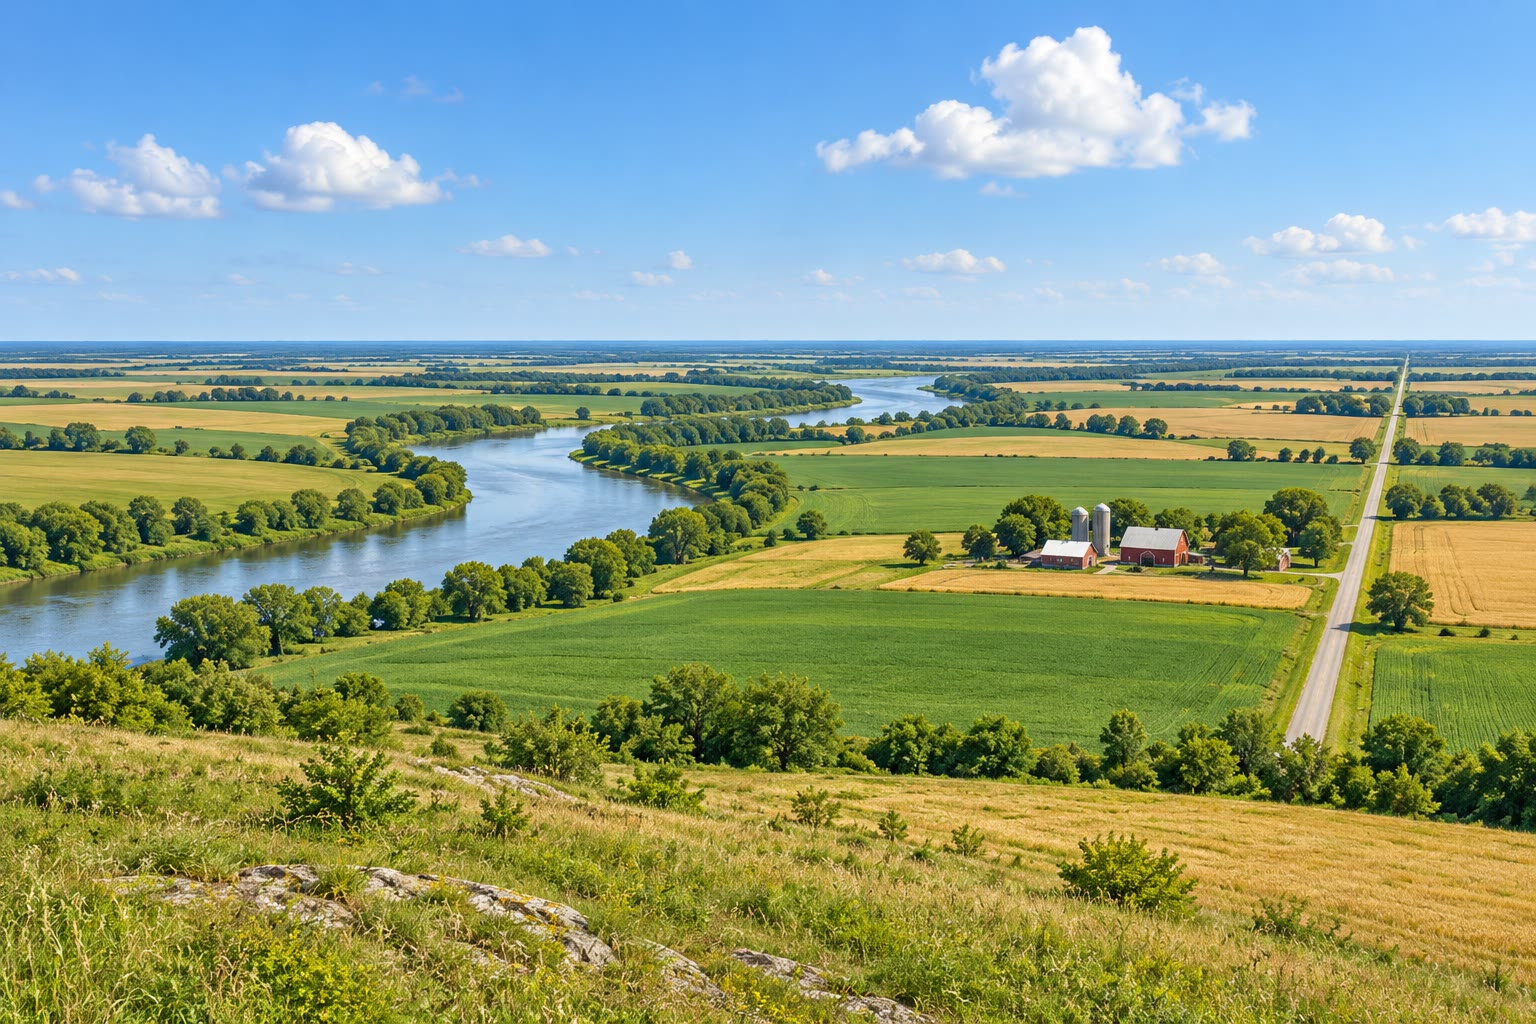
\includegraphics[width=\linewidth]{images/book1/ai/g1-plain-river.jpg}

{\small A \omterm{def:g1:landscapes-around-us:landform}{plain}, with a \omterm{def:g1:landscapes-around-us:water}{river} and fields.}
\end{minipage}
\end{omfigure}

\begin{example}[Mountain or hill?]\label{ex:g1:landscapes-around-us:mountain-hill}
There is no exact height at which a \omterm{def:g1:landscapes-around-us:landform}{hill} becomes a \omterm{def:g1:landscapes-around-us:landform}{mountain}. We look at the
shape: a \omterm{def:g1:landscapes-around-us:landform}{mountain} is high and steep, often rocky, sometimes with snow on
top; a \omterm{def:g1:landscapes-around-us:landform}{hill} is lower and rounder, often covered with grass, fields or
woods, and we can walk to its top in a short time.
\end{example}

\section{Water in the landscape}

Water is part of most \omterm{def:g1:landscapes-around-us:landscape}{landscapes}. It flows down from the \omterm{def:g1:landscapes-around-us:landform}{hills} and the
\omterm{def:g1:landscapes-around-us:landform}{mountains}, gathers in hollows, and reaches the sea.

\begin{definition}[Water in a landscape]\label{def:g1:landscapes-around-us:water}
A \emph{river}\index{river} is water that flows all the time in a long
channel, from higher land down to a lake or to the sea. A
\emph{lake}\index{lake} is a large body of water surrounded by land. The
\emph{coast}\index{coast} is the place where the land meets the sea.
\end{definition}

\begin{omfigure}
\begin{minipage}[b]{0.49\linewidth}\centering
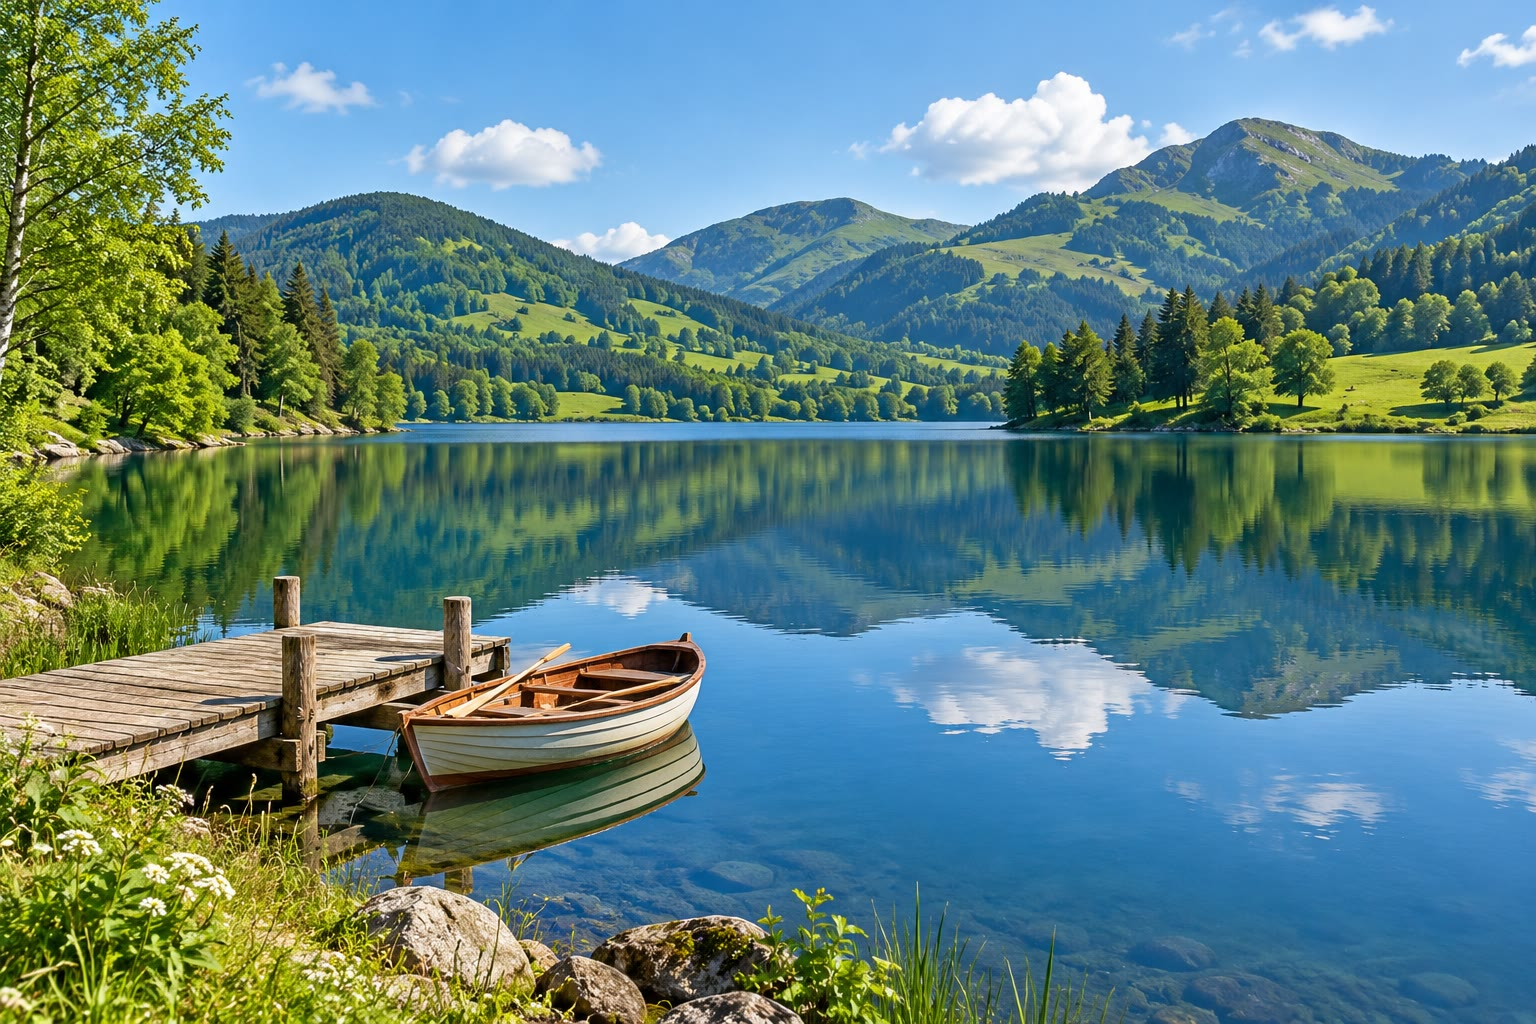
\includegraphics[width=\linewidth]{images/book1/ai/g1-lake-hills.jpg}

{\small A \omterm{def:g1:landscapes-around-us:water}{lake} among \omterm{def:g1:landscapes-around-us:landform}{hills}.}
\end{minipage}\hfill
\begin{minipage}[b]{0.49\linewidth}\centering
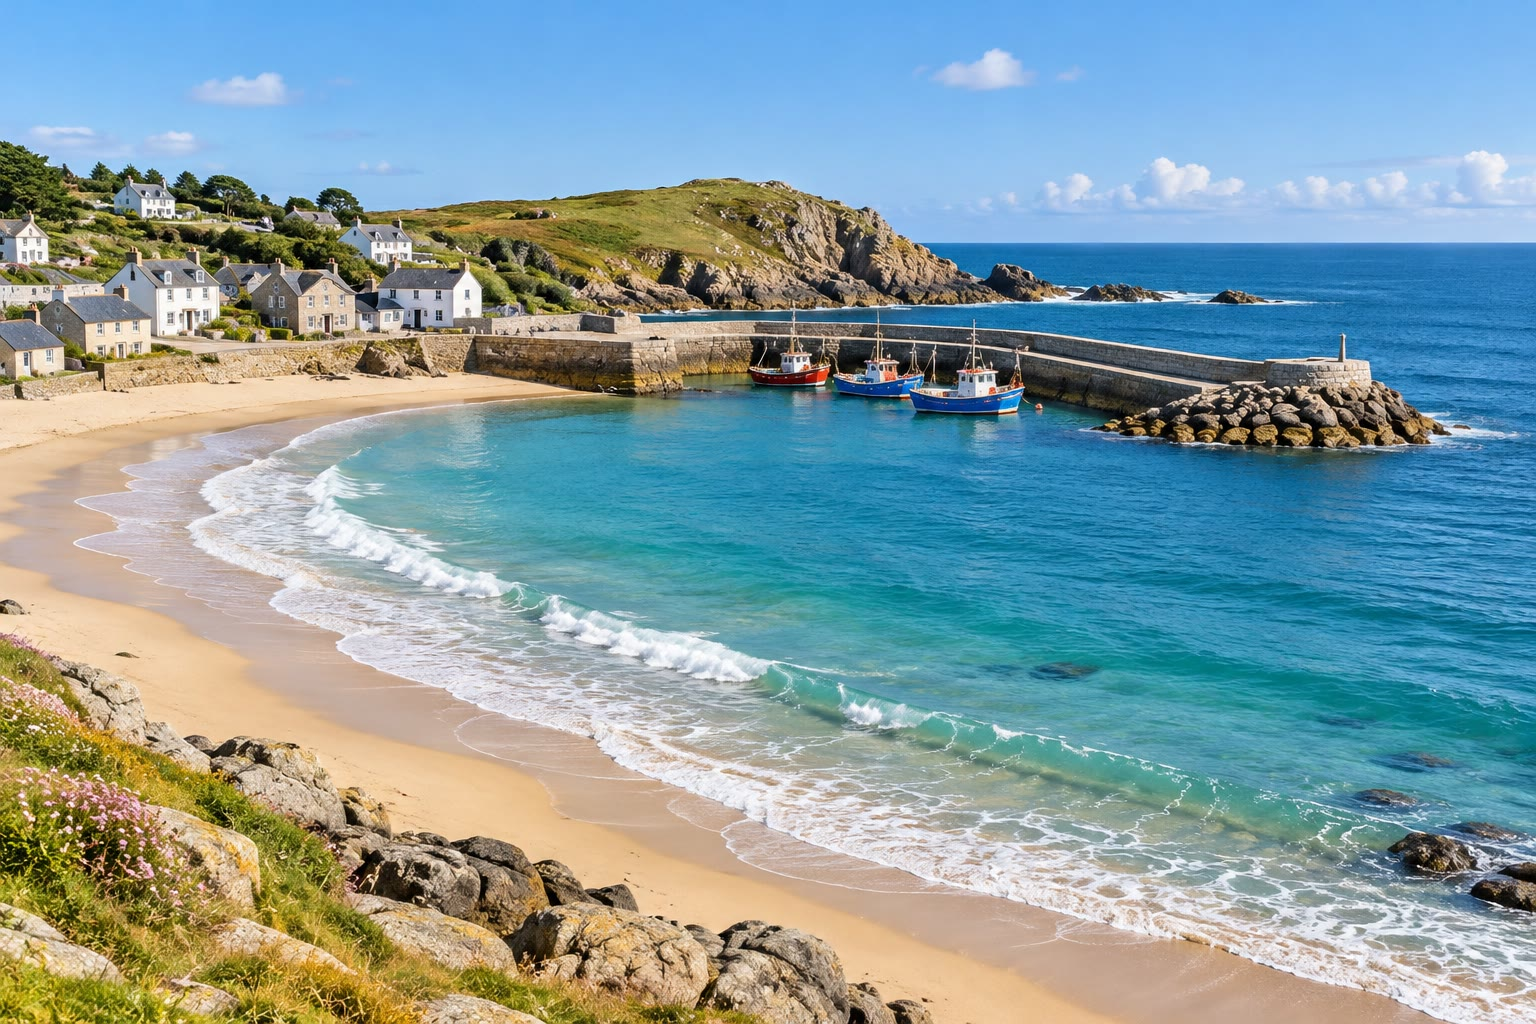
\includegraphics[width=\linewidth]{images/book1/ai/g1-coast-harbour.jpg}

{\small A \omterm{def:g1:landscapes-around-us:water}{coast}: a beach, rocks and a harbour.}
\end{minipage}
\end{omfigure}

\begin{remark}[Water always runs downhill]\label{rem:g1:landscapes-around-us:downhill}
A \omterm{def:g1:landscapes-around-us:water}{river} always flows from higher ground to lower ground. That is why
\omterm{def:g1:landscapes-around-us:water}{rivers} run at the bottom of \omterm{def:g1:landscapes-around-us:landform}{valleys}, and why, in the end, they reach a \omterm{def:g1:landscapes-around-us:water}{lake}
or the sea, which are lower than the land around them.
\end{remark}

\section{Natural parts and built parts}

Some parts of a \omterm{def:g1:landscapes-around-us:landscape}{landscape} were there before people came: the \omterm{def:g1:landscapes-around-us:landform}{mountains},
the \omterm{def:g1:landscapes-around-us:water}{rivers}, the forests. Other parts were made by people: houses, roads,
bridges, fields.

\begin{definition}[Natural and built parts]\label{def:g1:landscapes-around-us:natural-built}
A \emph{natural element}\index{natural element} of a \omterm{def:g1:landscapes-around-us:landscape}{landscape} is a part
that was not made by people: a \omterm{def:g1:landscapes-around-us:landform}{mountain}, a \omterm{def:g1:landscapes-around-us:water}{river}, a \omterm{def:g1:landscapes-around-us:water}{lake}, a forest, a beach.
A \emph{built element}\index{built element} is a part made or shaped by
people: a house, a road, a bridge, a harbour, a field, a garden.
\end{definition}

\begin{omfigure}
\begin{tikzpicture}[x=1cm, y=1cm]
  \node[draw=omDef!80!black, fill=omDef!10, rounded corners, text width=5.2cm,
        align=left, minimum height=3.2cm, anchor=north] (n) at (0,0)
    {\textbf{natural}\\[2pt] mountain\\ hill\\ valley\\ river\\ lake\\ forest\\ beach};
  \node[draw=omMeth!80!black, fill=omMeth!10, rounded corners, text width=5.2cm,
        align=left, minimum height=3.2cm, anchor=north] (b) at (6,0)
    {\textbf{built by people}\\[2pt] house\\ church\\ road\\ bridge\\ harbour\\ field\\ garden};
\end{tikzpicture}

{\small Sorting the parts of Mia's \omterm{def:g1:landscapes-around-us:landscape}{landscape}. A field is built: people
cleared the land and planted it.}
\label{fig:g1:landscapes-around-us:sort}
\end{omfigure}

\section{Landscapes change}

A \omterm{def:g1:landscapes-around-us:landscape}{landscape} is not the same for ever. Some changes are quick, and some are
so slow that nobody sees them in a lifetime.
\begin{itemize}
  \item \textbf{With the seasons:} the fields are brown after ploughing,
        green in spring, golden before the harvest; the trees lose their
        leaves in autumn; snow can cover everything in winter.
  \item \textbf{Because of people:} a village grows into a town; a forest
        is cut down to make fields; a new road and a bridge cross the
        \omterm{def:g1:landscapes-around-us:landform}{valley}.
  \item \textbf{Because of water and \omterm{def:g1:watching-the-weather:weather}{weather}:} after a great storm, a \omterm{def:g1:landscapes-around-us:water}{river}
        may leave its bed and cover the fields for a few days; on the
        \omterm{def:g1:landscapes-around-us:water}{coast}, the waves slowly wear the rocks away.
\end{itemize}

\begin{omfigure}
\begin{tikzpicture}[x=1cm, y=1cm]
  \foreach \k/\t in {0/long ago, 1/today} {
  \begin{scope}[shift={(\k*6.4,0)}]
    \fill[ocBlue!8] (0,0) rectangle (5.8,3.4);
    \fill[green!30!omLithAlluv] (0,0) rectangle (5.8,1.9);
    % river
    \fill[omSea] (0,0.55) .. controls (1.5,0.9) and (2.5,0.2) .. (5.8,0.6)
       -- (5.8,0.85) .. controls (2.5,0.45) and (1.5,1.15) .. (0,0.8) -- cycle;
    % hill
    \fill[green!45!black!55] (2.8,1.9) .. controls (3.8,3.1) and (4.8,3.1) .. (5.8,2.2) -- (5.8,1.9) -- cycle;
    \ifnum\k=0
      % forest everywhere, a few houses
      \foreach \x in {0.4,0.9,1.4,1.9,2.4,4.3,4.8,5.3}
        \fill[green!40!black] (\x,1.45) circle (0.22);
      \foreach \x in {3.4,3.75} {
        \fill[white, draw=black!50, line width=0.3pt] (\x,1.15) rectangle ++(0.24,0.2);
        \fill[red!60] (\x-0.03,1.35) -- ++(0.15,0.14) -- ++(0.15,-0.14) -- cycle; }
    \else
      % fields, many houses, a road and a bridge
      \foreach \x/\c in {0.1/yellow!60, 1.3/green!55, 4.5/yellow!45}
        \fill[\c] (\x,1.05) rectangle ++(1.1,0.5);
      \fill[black!35] (2.65,0) rectangle (2.95,1.9);
      \fill[black!55] (2.55,0.5) rectangle (3.05,0.9);
      \foreach \x in {3.2,3.55,3.9} \foreach \y in {1.1,1.45} {
        \fill[white, draw=black!50, line width=0.3pt] (\x,\y) rectangle ++(0.24,0.2);
        \fill[red!60] (\x-0.03,\y+0.2) -- ++(0.15,0.14) -- ++(0.15,-0.14) -- cycle; }
      \foreach \x in {4.6,5.2} \fill[green!40!black] (\x,2.35) circle (0.2);
    \fi
    \node[font=\small\bfseries] at (2.9,-0.3) {\t};
  \end{scope}}
\end{tikzpicture}

{\small The same \omterm{def:g1:landscapes-around-us:landform}{valley} long ago and today. The \omterm{def:g1:landscapes-around-us:landform}{hill} and the \omterm{def:g1:landscapes-around-us:water}{river} have not
moved; people have cut most of the forest, made fields, built more houses,
a road and a bridge.}
\label{fig:g1:landscapes-around-us:change}
\end{omfigure}

\begin{example}[Town and countryside]\label{ex:g1:landscapes-around-us:town}
In a town, almost everything we see was built: streets, houses, shops,
bridges, parks. In the countryside we see mostly fields, woods and
meadows, with a few farms and villages. Both are \omterm{def:g1:landscapes-around-us:landscape}{landscapes}. Even in the
middle of a big town the shapes of the land are still there: a \omterm{def:g1:landscapes-around-us:water}{river}
crosses the town, and some streets climb up a \omterm{def:g1:landscapes-around-us:landform}{hill}.
\end{example}

\section{Describing a landscape}

\begin{method}[Describing a landscape in four steps]\label{met:g1:landscapes-around-us:describe}
To describe a \omterm{def:g1:landscapes-around-us:landscape}{landscape}, from a hilltop or from a picture:
\begin{enumerate}
  \item \textbf{Split it into three bands:} the foreground, the middle
        ground and the background.
  \item \textbf{Name the shapes of the land:} \omterm{def:g1:landscapes-around-us:landform}{mountains}, \omterm{def:g1:landscapes-around-us:landform}{hills}, \omterm{def:g1:landscapes-around-us:landform}{valleys},
        \omterm{def:g1:landscapes-around-us:landform}{plains}.
  \item \textbf{Find the water:} a \omterm{def:g1:landscapes-around-us:water}{river}, a \omterm{def:g1:landscapes-around-us:water}{lake}, the sea and its \omterm{def:g1:landscapes-around-us:water}{coast}.
  \item \textbf{Find what people have built:} houses, roads, bridges,
        fields.
\end{enumerate}
\end{method}

\begin{example}[Mia's landscape]\label{ex:g1:landscapes-around-us:mia}
In the foreground, the grass at the top of the \omterm{def:g1:landscapes-around-us:landform}{hill}. In the middle ground,
a \omterm{def:g1:landscapes-around-us:landform}{valley} with a \omterm{def:g1:landscapes-around-us:water}{river}, a bridge and a village, fields around it, and a
forest on the next \omterm{def:g1:landscapes-around-us:landform}{hill}. In the background, a \omterm{def:g1:landscapes-around-us:landform}{plain} and, at the end of the
land, the \omterm{def:g1:landscapes-around-us:water}{coast} and the sea. Natural: the \omterm{def:g1:landscapes-around-us:landform}{hills}, the \omterm{def:g1:landscapes-around-us:landform}{valley}, the \omterm{def:g1:landscapes-around-us:water}{river}, the
forest, the sea. Built: the village, the church, the bridge, the fields.
\end{example}

\section{Exercises}

\begin{exercise}[$\star$]\label{exo:g1:landscapes-around-us:1}
Name the four shapes of the land you have learnt in this chapter.
\end{exercise}

\begin{exercise}[$\star$]\label{exo:g1:landscapes-around-us:2}
Which is higher and steeper: a \omterm{def:g1:landscapes-around-us:landform}{hill} or a \omterm{def:g1:landscapes-around-us:landform}{mountain}?
\end{exercise}

\begin{exercise}[$\star$]\label{exo:g1:landscapes-around-us:3}
Natural or built? A \omterm{def:g1:landscapes-around-us:water}{river}; a road; a forest; a bridge; a beach; a house.
\end{exercise}

\begin{exercise}[$\star$]\label{exo:g1:landscapes-around-us:4}
Where is the \omterm{def:g1:landscapes-around-us:water}{coast}: where the land meets a \omterm{def:g1:landscapes-around-us:water}{river}, or where the land meets
the sea?
\end{exercise}

\begin{exercise}[$\star$]\label{exo:g1:landscapes-around-us:5}
Look at the picture of the \omterm{def:g1:landscapes-around-us:landform}{mountains} and their village. Name one \omterm{def:g1:landscapes-around-us:natural-built}{natural
element} and one \omterm{def:g1:landscapes-around-us:natural-built}{built element}.
\end{exercise}

\begin{exercise}[$\star$]\label{exo:g1:landscapes-around-us:6}
On the drawing of the shapes of the land, which \omterm{def:g1:landscapes-around-us:landform}{landform} is the highest?
Where does the \omterm{def:g1:landscapes-around-us:water}{river} flow?
\end{exercise}

\begin{exercise}[$\star\star$]\label{exo:g1:landscapes-around-us:7}
Where does a \omterm{def:g1:landscapes-around-us:water}{river} flow from, and where does it go? Why does it never flow
up to the top of a \omterm{def:g1:landscapes-around-us:landform}{hill}?
\end{exercise}

\begin{exercise}[$\star\star$]\label{exo:g1:landscapes-around-us:8}
In a picture of a \omterm{def:g1:landscapes-around-us:landscape}{landscape}, a tree at the bottom of the picture looks
bigger than a whole \omterm{def:g1:landscapes-around-us:landform}{hill} at the top. Why?
\end{exercise}

\begin{exercise}[$\star\star$]\label{exo:g1:landscapes-around-us:9}
Describe the picture of the \omterm{def:g1:landscapes-around-us:landform}{plain} with its \omterm{def:g1:landscapes-around-us:water}{river} in three bands: what is
in the foreground, in the middle ground and in the background?
\end{exercise}

\begin{exercise}[$\star\star$]\label{exo:g1:landscapes-around-us:10}
A field of wheat is green or golden, like grass. Why do we say it is a
\omterm{def:g1:landscapes-around-us:natural-built}{built element} of the \omterm{def:g1:landscapes-around-us:landscape}{landscape} and not a natural one?
\end{exercise}

\begin{exercise}[$\star\star$]\label{exo:g1:landscapes-around-us:11}
Look at the drawing of the \omterm{def:g1:landscapes-around-us:landform}{valley} long ago and today. Name two things that
have not changed and three things that people have added.
\end{exercise}
